\documentclass[10pt]{article}
\usepackage[margin=0.8in]{geometry}
\usepackage{amsmath,amssymb}
\usepackage{booktabs}
\usepackage{graphicx}
\usepackage{caption}
\usepackage[colorlinks=true,linkcolor=blue,citecolor=blue,urlcolor=blue]{hyperref}
\usepackage{titlesec}
\usepackage{enumitem}
\usepackage{fancyhdr}
\usepackage{float}

\captionsetup{font=small,labelfont=bf}
\titleformat{\section}{\normalfont\large\bfseries}{\thesection}{0.6em}{}
\titlespacing*{\section}{0pt}{6pt}{3pt}
\setlist{itemsep=1pt,parsep=0pt,topsep=2pt}
\setlength{\parskip}{1pt}

\pagestyle{fancy}
\fancyhf{}
\rhead{\small Kahlus --- metric inflation in windowed forecast evaluation, 30 July 2026}
\cfoot{\thepage}
\renewcommand{\headrulewidth}{0.4pt}

\begin{document}

\begin{center}
{\LARGE\bfseries A closed-form bound on metric inflation\\[2pt]
in windowed forecast evaluation}\\[7pt]
{\large And a corrected, powered EEG forecasting benchmark}\\[10pt]
{\normalsize Kahlus / Neural-CASP}\\[5pt]
{\small 30 July 2026}\\[3pt]
{\small Repository \texttt{Kahlus-V1}, branches
\texttt{finding/overlap-inflation-law}, \texttt{finding/forecast-crossover-f8}}
\end{center}

\vspace{2pt}\hrule\vspace{5pt}

\begin{quote}\small
\textbf{Scope.} Three results: an exact bound on how much a window-scored
forecast metric can overstate forecast skill --- derived, not fitted, and violated
by no $(W,H)$ pair on any trace we tested; the corresponding result for
\emph{correlation}, which turns out \emph{not} to inherit the same constant, so
the convenient extrapolation is falsified here rather than left to a reader; and
a corrected benchmark that survived eight falsification tests, one of which
broke a secondary claim we had made. Both failures are reported rather than
removed. Every number is traceable to a named artifact.
\end{quote}

\vspace{2pt}

\section{The problem}

A forecasting task is only a forecast if the target does not contain the input.
The construction below is common in the biosignal literature and violates that
silently. From a sequence of length $W{+}H$:
\[
X = \mathrm{seq}[0\!:\!W], \qquad Y = \mathrm{seq}[H\!:\!H{+}W].
\]
Then $Y[k] = X[k{+}H]$ whenever $k < W{-}H$: of the $W$ scored target positions,
$W{-}H$ are \textbf{copyable} --- literally present in the input at a shifted index
--- and only $H$ are strictly future. Averaging over all $W$ positions therefore
dilutes a genuine forecast error with positions a model can copy.

This is not the leakage the field guards against. It survives subject-wise
partitioning, nested cross-validation and non-overlapping strides, because it lives
\emph{inside a single training example} rather than across the train/test split ---
and the leakage literature we could find (Bernett et al., \textit{Nat.\ Methods}
2024; Del Pup et al.\ 2025, five CV schemes over $10^5$ trained EEG models;
Apicella et al.\ 2024) treats only information shared \emph{between} examples.

\section{The law}

Score \textbf{one model's one set of predictions} under three masks --- all
positions, the copyable prefix, the strictly-future tail. No argument about
capacity, training or tuning can explain a gap between them. By construction,
\[
\mathrm{MSE}_{\text{overlap}}
= \frac{(W{-}H)\,\mathrm{MSE}_{\text{copy}} + H\,\mathrm{MSE}_{\text{future}}}{W},
\]
an identity rather than a fit, which rearranges to
\[
\boxed{\;
\text{inflation} \;\equiv\;
\frac{\mathrm{MSE}_{\text{future}}}{\mathrm{MSE}_{\text{overlap}}}
\;=\;
\frac{W/H}{\,1 + \frac{W-H}{H}\cdot\frac{\mathrm{MSE}_{\text{copy}}}{\mathrm{MSE}_{\text{future}}}\,}
\;\le\; \frac{W}{H}. \;}
\]
Equality holds as $\mathrm{MSE}_{\text{copy}}\!\to\!0$. The bound is one-sided: a
real result can never exceed it, so $W/H$ is always safe as a worst case.

\textbf{$W/H$ requires no data} --- only the window length and horizon printed in
a methods section. A paper reporting a 128-sample target window at horizon 1 is
reporting a number that may be up to $128\times$ better than its forecast error.

\begin{figure}[tb]
\centering
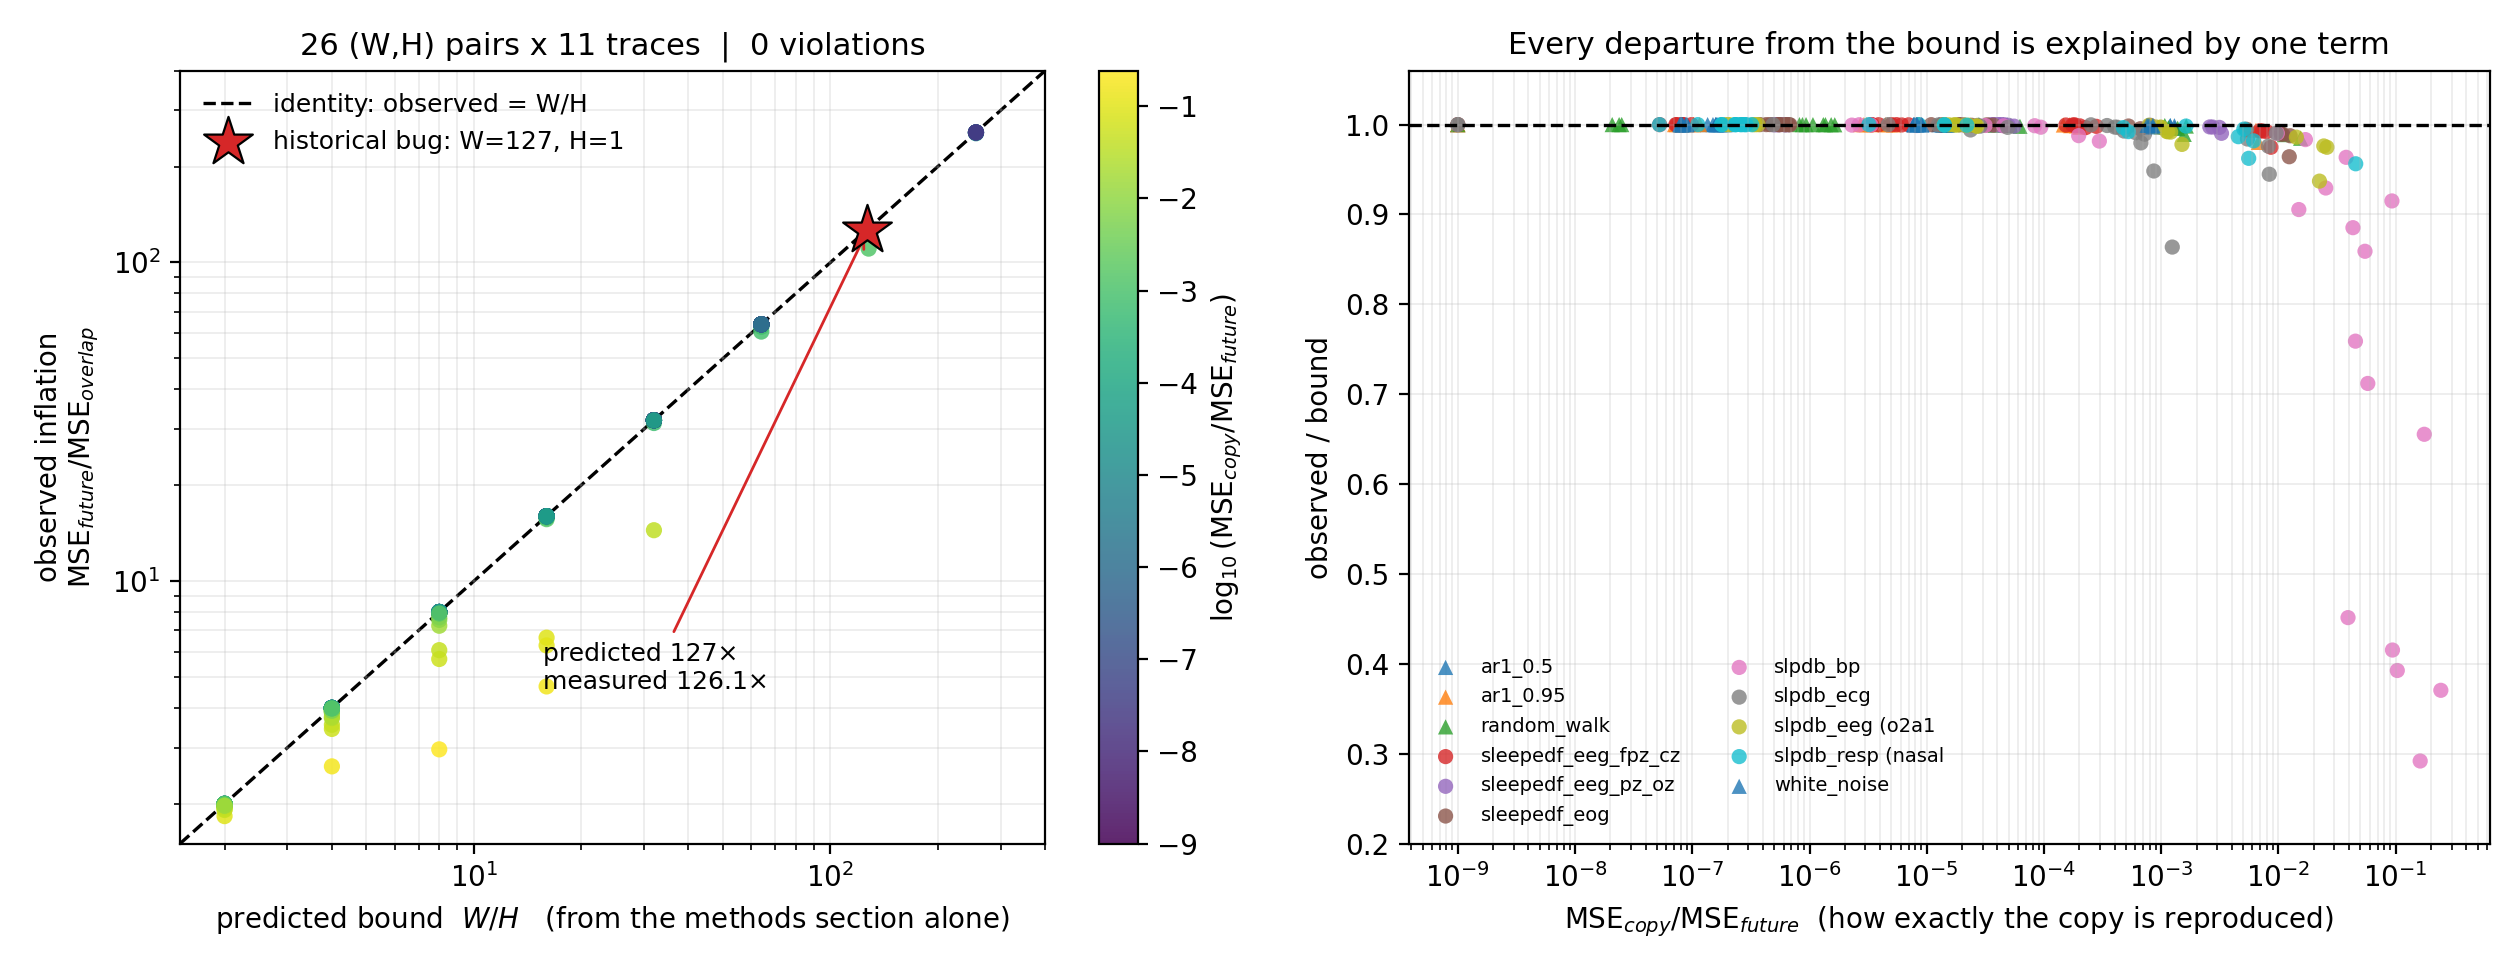
\includegraphics[width=0.88\textwidth]{overlap_law.png}
\caption{\textbf{Left:} predicted bound $W/H$ against observed MSE inflation,
log--log. Points lie on the identity and never above it; the region where a
counterexample would appear is empty. The star is this project's own invalidated
result ($W{=}127$, $H{=}1$): predicted $127\times$, measured $126.1\times$.
\textbf{Right:} every departure is explained by the single term
$\mathrm{MSE}_{\text{copy}}/\mathrm{MSE}_{\text{future}}$, monotonically, across
five decades. Triangles synthetic, circles real recordings.}
\end{figure}

\section{The same question for correlation, and a negative answer}

Most work in this area leads with $r$, not MSE, so whether $W/H$ transfers
decides how far the bound reaches. Correlation is a ratio, not a per-position
average, so the identity above does not apply. An AM-GM argument on the pooled
deviation moments still gives an exact, assumption-free bound,
\[
|r_{\text{overlap}}| \;\le\; \bigl|\,\mu\, r_{\text{copy}} + (1-\mu)\, r_{\text{future}}\bigr|,
\]
with $\mu$ the variance share of the copyable positions --- a reported
correlation is at most a variance-weighted blend of how well a model copies and
how well it forecasts. Violated by none of the 286 cells.

\textbf{But $W/H$ does not carry over.} Expanding $\mu$ gives the exact
correlation-gap bound $1 + \frac{W-H}{H}(s_{p}s_{t})^{-1/2}$, where $s_p, s_t$
are the future/copy per-position variance ratios of the prediction and target;
$W/H$ is only the case $s_p{=}s_t{=}1$. Targets are variance-stationary
($s_t$ median $0.996$), but predictions are not: a regularised model shrinks
toward the mean precisely where the signal is unpredictable ($s_p$ median
$0.700$). So the true deflation \emph{exceeds} $W/H$ --- median $1.21\times$, up
to $10.8\times$ --- on \textbf{223 of 286 cells}, always in the direction that
flatters the paper, and worst where there is least real signal. The shrinkage
form reproduces the measured bound to median relative error $7.1\times10^{-16}$,
so this is a mechanism, not an anomaly. \textbf{The sharpest case is white
noise at $W{=}32, H{=}1$: reported $r=0.984$, true $r_{\text{future}}=0.014$.}

What survives with no data is one-directional: $r < 1-H/W$ proves a reported
correlation bounds nothing; clearing that screen does not prove it informative.

\begin{figure}[htb]
\centering
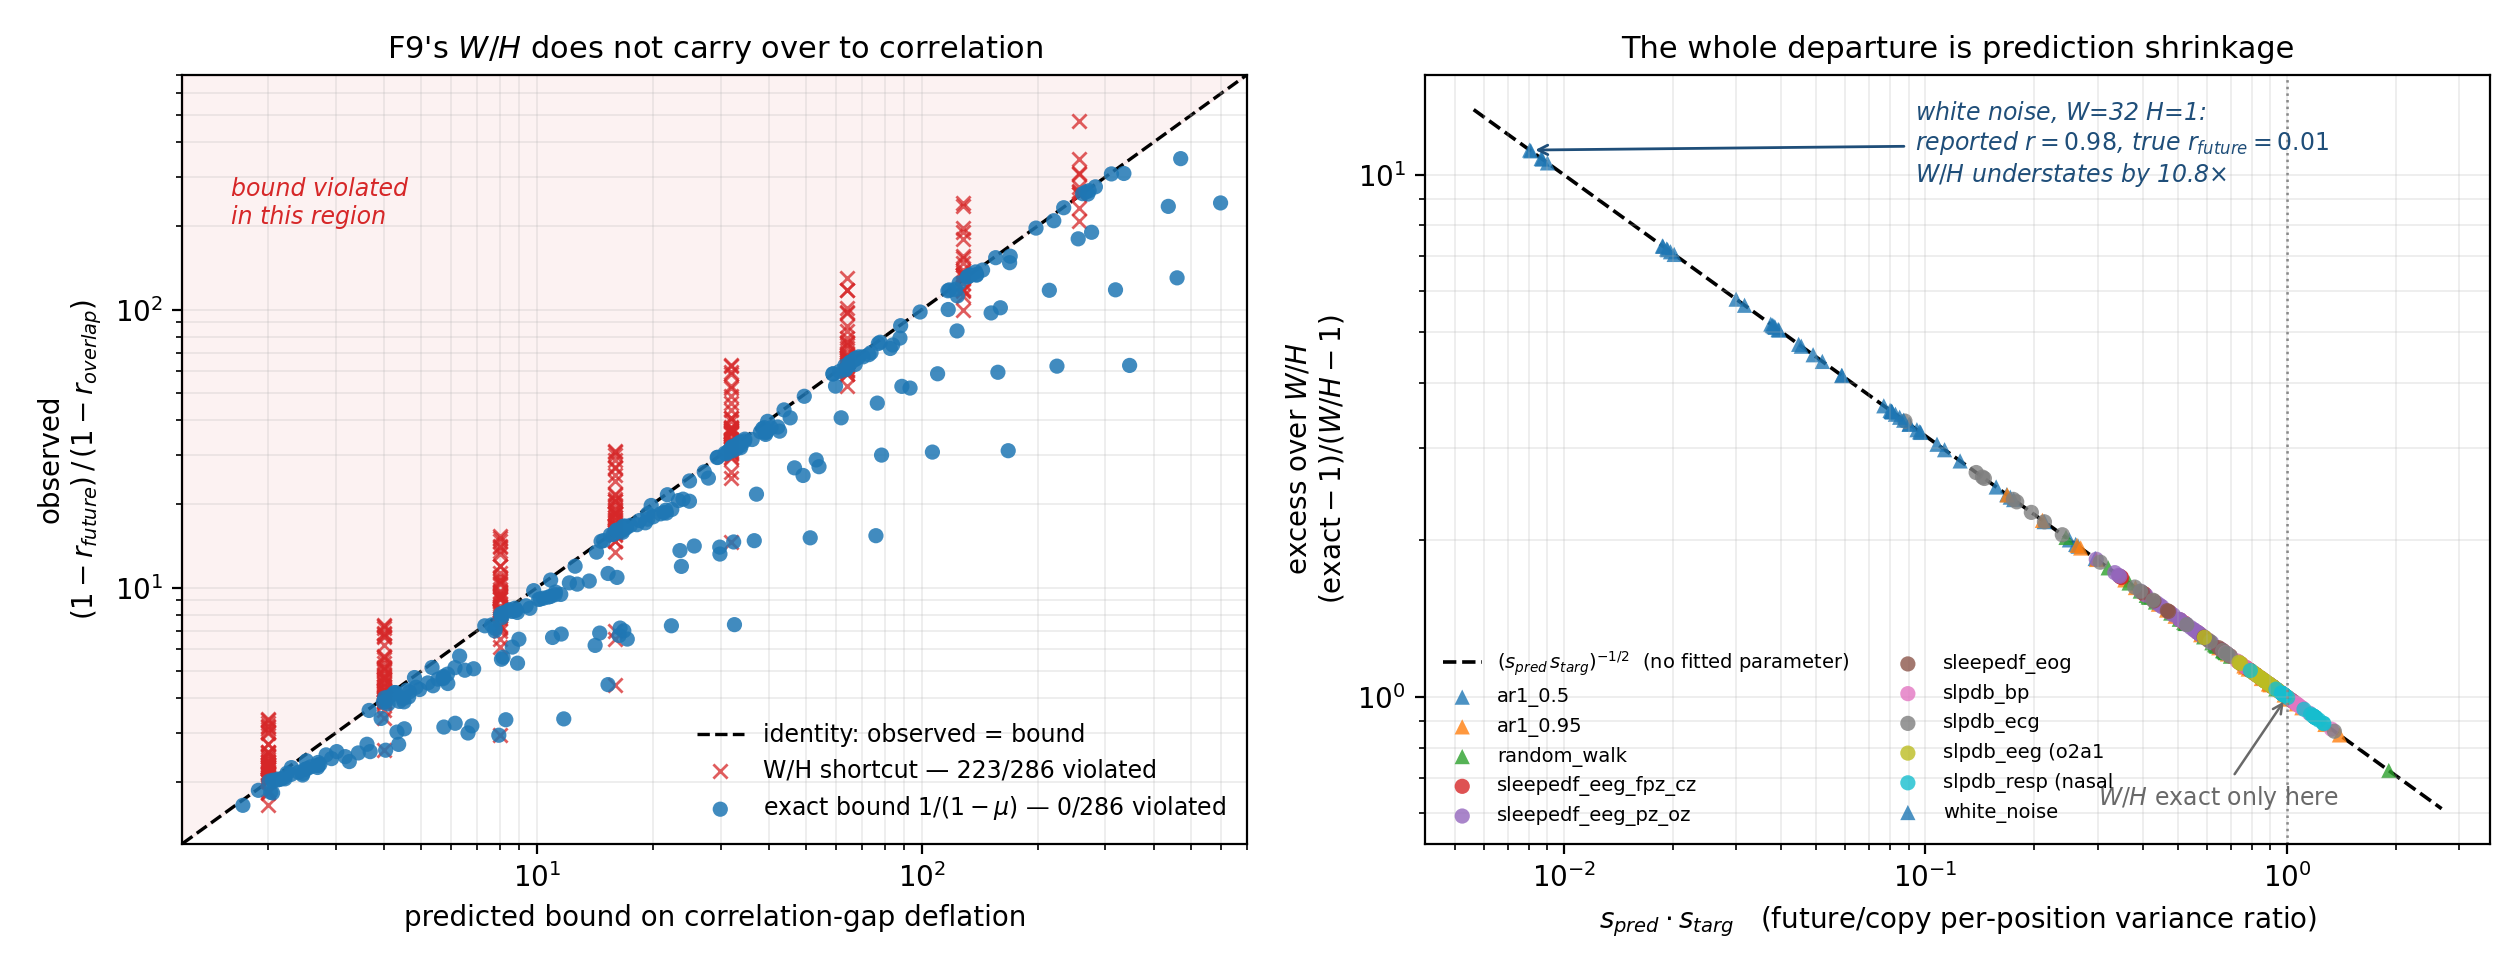
\includegraphics[width=0.88\textwidth]{correlation_law.png}
\caption{\textbf{Left:} the exact correlation bound is violated by none of the
286 cells; the $W/H$ shortcut carried over from the MSE law is violated by 223,
all of them in the shaded region where a reported number looks better than it
is. \textbf{Right:} the departure is not noise. Rearranging the exact bound
forces $(\text{exact}-1)/(W/H-1) = (s_p s_t)^{-1/2}$ with no fitted parameter,
and every cell lies on that curve across three decades. $W/H$ is correct only
where the dotted line crosses it --- i.e.\ only for a model that does not shrink.}
\end{figure}

\section{Verification}

Both laws are checked on the same 26-point grid,
$W\in\{32,64,128,256\}\times H\in\{1,\dots,128\}$ with $H<W$, over 11 traces:
\textbf{7 recorded channels} from Sleep-EDF (Fpz-Cz, Pz-Oz, EOG) and MIT-BIH
polysomnographic (ECG, blood pressure, O2-A1 EEG, nasal respiration), plus 4
synthetic processes (white noise, AR(1) $\phi{\in}\{0.5,0.95\}$, random walk) ---
picked for spread in autocorrelation rather than for count.

\vspace{1pt}
\noindent\textbf{No $(W,H)$ pair violated either exact bound, on any trace}
(286 grid cells). For the MSE law, observed/bound median $1.000$, mean $0.981$,
matching the exact formula to a maximum relative error of $1.3\times10^{-15}$ ---
machine precision, because the relation is an identity, and the code asserts the
decomposition per cell so an incorrect mask fails loudly rather than producing a
plausible curve. Departures are monotone in the correction term: the law is not
approximately right by luck, it is exactly right with a known correction. White
noise, where nothing whatever is predictable, still inflates at the bound --- the
artifact belongs to the \emph{metric}, not to the signal or the model.

\section{The corrected benchmark}

Strictly-future scoring on real data: Sleep-EDF sleep-cassette, all 78 subjects,
subject-disjoint 39\,/\,12\,/\,27, zero input--target overlap. Both models tuned per
horizon on the same validation subjects, the ridge grid extended until no horizon
selected a grid edge. Per-subject MSE, paired Wilcoxon, Holm-corrected across nine
horizons.

\begin{center}\small
\begin{tabular}{rrrrrrr}
\toprule
$h$ & ms & persistence & ridge-AR & GRU & $\Delta$ & Holm $p$ \\
\midrule
16 & 160 & 1.3814 & 0.8298 & \textbf{0.7268} & $\mathbf{+0.1031}$ & $\mathbf{2.2\times10^{-6}}$ \\
32 & 320 & 1.7600 & \textbf{0.8700} & 0.8756 & $-0.0056$ & n.s. \\
256 & 2560 & 1.8746 & \textbf{0.9942} & 1.0099 & $-0.0157$ & $1.3\times10^{-7}$ \\
\bottomrule
\end{tabular}
\end{center}

At 160\,ms the GRU is 12.4\,\% below a converged linear baseline on 26 of 27
held-out subjects and 47.4\,\% below persistence; the advantage ends by
$\sim$320\,ms. Eight falsification tests followed. Two matter most: on a synthetic
AR(2) process, where the optimal predictor is provably linear, the same GRU with
the same tuning budget \textbf{loses} to ridge ($p{=}0.014$), so the apparatus
cannot manufacture wins; and a linear model trained by the GRU's exact optimiser
is \emph{worse} than closed-form ridge at every horizon, so the margin is
architecture, not optimisation. \textbf{One claim did not survive:} we had reported
tuned ridge beating the GRU at 640\,ms ($p{=}4.1\times10^{-5}$), but under
non-overlapping windows that becomes a tie ($p{=}0.58$), so the claim is narrowed
to ``the advantage ends by 320\,ms'' rather than ``linear wins beyond it''.

\vspace{2pt}\hrule\vspace{3pt}
\noindent\small
\textbf{Not claimed.} No clinical utility --- 160\,ms is roughly $400\times$ shorter
than the $\sim$1\,minute precursor timescale of interest. Single channel, one
corpus. The prevalence survey, establishing how often published work uses $H<W$,
is not done; that is what would turn these from tools for auditing one paper
into a finding about the field.

\vspace{3pt}
\noindent\scriptsize
\textbf{Artifacts.} \texttt{artifacts/\{overlap\_law, correlation\_law,
forecast\_crossover\}/} hold the cells, figures, benchmark and the eight-test
validation, each beside its write-up in \texttt{docs/results/}. Produced by
\texttt{scripts/\{overlap\_inflation\_law, correlation\_inflation\_law,
forecast\_scaleup\_paired, validate\_forecast\_claim\}.py}; the correlation
harness carries a \texttt{--selftest} for the theorem. The invalidated
$3.116$\,MSE\,/\,$r{=}0.972$ result is retained in
\texttt{docs/results/a100-run-history.md} as evidence of the bug, not as
performance --- note it fails the $r<1-H/W$ screen, so it never bounded forecast
skill at all.

\end{document}
